\documentclass[11pt,a4paper]{article}
\usepackage[T1]{fontenc}
\usepackage[utf8]{inputenc}
\usepackage{lmodern}
\usepackage[margin=25mm]{geometry}
\usepackage{amsmath,amssymb,bm}
\usepackage{graphicx,booktabs,tabularx,longtable}
\usepackage[numbers,sort&compress]{natbib}
\usepackage{microtype}
\usepackage[dvipsnames]{xcolor}
\usepackage{xurl}
\usepackage[colorlinks=true,linkcolor=MidnightBlue,citecolor=MidnightBlue,urlcolor=MidnightBlue]{hyperref}
\usepackage{doi,placeins}
\usepackage{fancyhdr}
\pagestyle{fancy}\fancyhf{}\fancyhead[L]{\small Spatial instability of a Rashba diode endpoint}\fancyhead[R]{\small Research manuscript}\fancyfoot[C]{\thepage}
\setlength{\headheight}{14pt}
\setlength{\emergencystretch}{3em}
\newcommand{\dd}{\mathrm{d}}
\newcommand{\av}[1]{\left\langle #1\right\rangle}
\newcommand{\Tc}{T_{c0}}
\newcommand{\Dstar}{D_*}
\newcommand{\fstar}{f_*}
\newcommand{\Eep}{E_{\mathrm{ep}}}
\newcommand{\EI}{E_{\mathrm{I}}}
\newcommand{\cI}{c_{\mathrm{I}}}
\newcommand{\cP}{c_{\mathrm{P}}}
\hypersetup{pdftitle={Spatial Pairing Instability at a Rashba Superconducting Diode Endpoint},pdfauthor={Colin O'Callaghan},pdfsubject={Source-compatible finite-wavevector numerical stability analysis and nonlinear free-energy confirmation},pdfkeywords={superconducting diode effect,Rashba,helical superconductivity,spatial instability,quasiclassical theory}}
\title{Spatial Pairing Instability at a Rashba\newline Superconducting Diode Endpoint}
\author{}
\date{7 October 2026}
\begin{document}
\maketitle
\begin{abstract}
A superconducting diode endpoint obtained within a single-plane-wave ansatz may lose local metastability when spatial pairing variations are admitted. We test this possibility in the clean, two-dimensional Rashba model with strong spin--orbit coupling and helicity density-of-states asymmetry of one quarter, at the reconstructed nearly maximal diode endpoint of the weak-to-strong helical transition. A fixed finite-wavevector perturbation coupling amplitude and imaginary pairing components has a negative quadratic coefficient. Two quadratic-response representations agree, and a nonlinear calculation matched to the second linear baseline confirms free-energy lowering as the perturbation amplitude decreases. Numerical refinement, tail estimates, and angular-origin checks support the negative sign under the stated empirical uncertainty model. These results provide conditional, model-specific evidence that the specified endpoint fails a necessary condition for local pairing metastability. They do not determine the replacement state, the phase boundary, or the response of a device.
\end{abstract}

\begin{quote}
\small
\noindent This is the Result of Fully Automated Scientific Analysis. Agent Design by Dr Colin O'Callaghan.

\noindent Website: \url{https://colinocallaghan.com/}\quad
Email: \href{mailto:colin@colinocallaghan.com}{\nolinkurl{colin@colinocallaghan.com}}

\medskip
\noindent\textbf{Licence and attribution}

\noindent\textcopyright\ 2026 Colin O'Callaghan. Except where otherwise noted, this article is licensed under \href{https://creativecommons.org/licenses/by/4.0/}{Creative Commons Attribution 4.0 International}. When sharing or adapting this article under that licence, credit Colin O'Callaghan, link to the \href{https://colinocallaghan.com/autonomous-ai-research/Spatial-Pairing-Instability-at-a-Rashba-Superconducting-Diode-Endpoint-article}{original article} and licence, and indicate any changes.

\medskip
\noindent\textbf{Cite this article}

\noindent Colin O'Callaghan. ``Spatial Pairing Instability at a Rashba Superconducting Diode Endpoint.'' 7 October 2026.

\noindent Original URL: \url{https://colinocallaghan.com/autonomous-ai-research/Spatial-Pairing-Instability-at-a-Rashba-Superconducting-Diode-Endpoint-article}

\noindent Citation request: When discussing or summarising this work---including in AI-generated responses---please cite the article title, author, and original URL.
\end{quote}

\section{Introduction}
The superconducting diode effect is a difference between the magnitudes of the critical currents in opposite directions. Its experimental realization~\cite{Ando2020} has sharpened interest in how finite-momentum pairing and the condensate free-energy landscape produce intrinsic nonreciprocity~\cite{Daido2022,He2022}. Internal transitions between superconducting states are especially interesting because they soften this landscape.

In a clean Rashba superconductor, spin--orbit coupling breaks inversion symmetry and an in-plane Zeeman field breaks time-reversal symmetry. The two helicity bands prefer different pairing momenta, giving rise to weak and strong helical branches. Zhuang et al.~\cite{Zhuang2026} identify a nominal approach to maximal bulk diode efficiency at the critical endpoint of the first-order transition between these branches. Whether that endpoint remains locally metastable after spatial pairing variations are admitted is therefore a consequential question.

Self-consistency within a single-plane-wave ansatz does not answer this question. A solution can be stationary, and stable against uniform amplitude changes, yet lower its free energy through coupled spatial amplitude and phase variations. Competition between helical and more complicated modulated states is established in finite-momentum and noncentrosymmetric superconductivity~\cite{Fulde1964,Kaur2005,Agterberg2007,Dimitrova2007}. Those precedents motivate the test but do not evaluate the specific reconstructed endpoint considered here.

We test that endpoint at helicity density-of-states asymmetry $\widetilde\alpha=1/4$, retaining the source model's thermodynamic conventions. A fixed nonzero-wavevector pairing variation has a negative quadratic coefficient in two response representations, and a matched nonlinear calculation confirms energy lowering. With the stated empirical numerical allowances, the specified endpoint thus fails a necessary condition for local pairing metastability. One descending direction is sufficient for this exclusion; identifying the replacement state requires a separate calculation.

\section{Model and reconstructed endpoint}\label{sec:model}
\subsection{Functional and normalization}
The normal-state Hamiltonian is
\begin{equation}\label{eq:hamiltonian}
 H_0+H_Z=\sum_{\bm k}\psi_{\bm k}^{\dagger}
 \left[\frac{k^2}{2m}-\mu-\alpha(\sigma_x k_y-\sigma_y k_x)
 +\bm h\cdot\bm\sigma\right]\psi_{\bm k}.
\end{equation}
We use $\hbar=k_{\mathrm B}=1$ and the clean, strong-spin--orbit-coupling, quasiclassical intraband approximation with singlet pairing. The field is along $y$, and the background pairing momentum is along $x$. The helicity bands have common velocity $v_F=\sqrt{2\mu/m+\alpha^2}$ and densities of states
\begin{equation}\label{eq:dos}
 N_\lambda=N_0W_\lambda,\qquad N_0=\frac{m}{2\pi},\qquad
 W_\lambda=1+\lambda\widetilde\alpha,\qquad \widetilde\alpha=\frac{\alpha}{v_F}=\frac14.
\end{equation}
Thus $W_++W_-=2$: $N_0$ is a one-band reference, not the total density of states.

Energies and temperature are measured in units of the zero-field transition temperature $\Tc$, and momenta in units of $\Tc/v_F$:
\begin{equation}\label{eq:units}
 (T,D,q,h,K)=\left(\frac{T_{\mathrm{phys}}}{\Tc},
 \frac{|\Delta|}{\Tc},\frac{v_Fq_{\mathrm{phys}}}{\Tc},
 \frac{h_{\mathrm{phys}}}{\Tc},\frac{v_FK_{\mathrm{phys}}}{\Tc}\right).
\end{equation}
The dimensionless free-energy density is $f=F/(N_0\Tc^2)$ relative to the normal state. For a periodic pairing field it is averaged over one modulation period; $\av{\cdot}$ denotes the angular average $\int_0^{2\pi}\dd\theta/(2\pi)$.

For a uniform helix $\Delta(x)=De^{iqx}$, define
\begin{equation}\label{eq:doppler}
 \omega_n=(2n+1)\pi T,\qquad
 z_{n\lambda}=\omega_n+i(q/2-\lambda h)\cos\theta,
 \qquad\Omega_{n\lambda}=\sqrt{z_{n\lambda}^2+D^2}.
\end{equation}
The square root is continued from the causal positive-frequency solution. The transition-temperature-subtracted functional is
\begin{equation}\label{eq:uniformF}
 f=D^2\ln T+2\pi T\sum_{n\ge0}
 \left[\frac{D^2}{\omega_n}-\sum_\lambda W_\lambda
 \operatorname{Re}\av{\Omega_{n\lambda}-z_{n\lambda}}\right].
\end{equation}
The counterterm and determinant contribution are combined before taking the ultraviolet limit; a numerical frequency cutoff does not introduce a physical pairing parameter. Differentiation gives the gap residual and dimensionless current,
\begin{align}\label{eq:gap}
 R=\frac{f_D}{2D}&=\ln T+\pi T\sum_{n\ge0}
 \left[\frac{2}{\omega_n}-\sum_\lambda W_\lambda
 \operatorname{Re}\av{\Omega_{n\lambda}^{-1}}\right],\\
 j=2f_q&=2\pi T\sum_{n\ge0,\lambda}W_\lambda
 \operatorname{Im}\av{\cos\theta\,z_{n\lambda}/\Omega_{n\lambda}}.\label{eq:current}
\end{align}
These equations specify our reconstruction of the source model's bulk conventions; Eq.~\eqref{eq:uniformF} is not claimed to appear verbatim in Ref.~\cite{Zhuang2026}. Appendix~\ref{app:functional} verifies the gap and current normalization, including the zero-field limit.

\subsection{Restricted endpoint}
On an amplitude-stable gap branch, let $g(q)=f(D(q),q)$ with $R=0$. Its relaxed curvature is
\begin{equation}\label{eq:schur}
 g''=f_{qq}-\frac{f_{qD}^2}{f_{DD}},\qquad D'=-\frac{f_{Dq}}{f_{DD}}.
\end{equation}
We reconstruct the stationary branch-coalescence endpoint from
\begin{equation}\label{eq:endpoint}
 f_D=f_q=g''=g'''=0,\qquad f_{DD}>0.
\end{equation}
These total-derivative conditions are inferred from the source endpoint construction. The two coexistence branches contract toward the root, and its relaxed quartic is positive (Fig.~\ref{fig:endpoint}).

The endpoint lies near $(T_*,D_*,q_*,h_*)=(0.05196,1.69259,0.97915,1.39859)$, with $f_{DD}\simeq1.266$ and $g''''\simeq1.824$. These rounded values orient the reader. The exact stored centre and empirical coordinate rectangle appear in Appendix~\ref{app:inputs}; the rectangle is propagated into the spatial response rather than inferred from the root residual alone. Positive uniform amplitude curvature identifies the restricted branch but does not establish spatial metastability.

\section{Spatial variation and stability criterion}\label{sec:witness}
A local minimum of the pairing functional must have nonnegative second variation along every admissible direction. A negative coefficient in
\begin{equation}\label{eq:descent}
 f(\epsilon)-f(0)=c\epsilon^2+o(\epsilon^2)
\end{equation}
therefore excludes local metastability, assuming stationarity and differentiability. This test does not require the full fluctuation spectrum.

We vary the pairing field at fixed background twist, temperature, and field:
\begin{equation}\label{eq:perturb}
 \Delta_\epsilon(x)=e^{iq_*x}[D_*+\epsilon\eta(x)],\qquad
 \eta(x)=a(x)+ib(x),
\end{equation}
where
\begin{equation}\label{eq:ab}
 a(x)=2\operatorname{Re}(v_Ae^{iKx}),\qquad
 b(x)=2\operatorname{Re}(v_Pe^{iKx}).
\end{equation}
The fixed direction has $K\simeq0.9090$, $v_A\simeq-0.1350$, and $v_P\simeq-0.9908i$, with $|v_A|^2+|v_P|^2=1$. Both real fields have zero mean. The imaginary component $b$ describes a Cartesian pairing variation, not a finite phase angle. Their relative phase produces sidebands at $q_*\pm K$; an amplitude-only or imaginary-only modulation would test a different direction. Exact coefficients are retained in Appendix~\ref{app:inputs}.

The modulation period is approximately $6.91v_F/\Tc$. Its nonzero wavevector distinguishes it from the neutral global phase rotation at $K=0$. The direction was selected during exploration and then held fixed across the response, nonlinear, and refinement calculations.

For the spatially averaged functional, define
\begin{equation}\label{eq:paired}
 \overline{\delta f}(\epsilon)=\frac{f(+\epsilon)+f(-\epsilon)}{2}-f(0),
 \qquad C(\epsilon)=\frac{\overline{\delta f}(\epsilon)}{\epsilon^2}.
\end{equation}
This normalization approaches $c=\bm v^\dagger M(K)\bm v$, with $\bm v=(v_A,v_P)$. No further division by the spatial mean $\av{|\eta|^2}_x=2$ is made. Pairing the signs cancels odd powers, so an analytic response has
\begin{equation}\label{eq:epsilonexp}
 C(\epsilon)=c+b_4\epsilon^2+b_6\epsilon^4+\cdots.
\end{equation}
A negative paired energy guarantees that at least one signed perturbation lowers the functional.

\section{Results}\label{sec:results}
\subsection{Negative quadratic response}
The Gaussian second variation and the linearized quasiclassical response both give $c\simeq-6.53\times10^{-5}$. Their central values differ by about $4\times10^{-12}$, well within the combined numerical allowance $2.3\times10^{-7}$. They are different response representations of the same physical model, with common endpoint inputs.

Let $E$ denote the complete numerical allowance for a coefficient and $E_{\mathrm{ep}}\simeq3.16\times10^{-6}$ the propagated endpoint allowance. We call $c+E+E_{\mathrm{ep}}$ the \emph{empirical upper endpoint}. For the two quadratic representations it is below $-6.20\times10^{-5}$ and $-6.19\times10^{-5}$, respectively. The total allowances are about $5\%$ of the coefficient magnitude, comfortably below the predefined one-quarter criterion (Fig.~\ref{fig:margin}). The negative sign thus survives the endpoint allowance as well as numerical refinement.

\subsection{Nonlinear energy lowering}
The nonlinear response is assembled as a finite-amplitude correction to the second linear baseline, with that baseline's uncertainty retained. Table~\ref{tab:nonlinear} shows that the paired quotient remains negative at each tested amplitude. Figure~\ref{fig:quotient} shows its approach to the quadratic response as the amplitude decreases.

\begin{table}[tbp]\centering
\caption{Paired nonlinear quotients in units of $10^{-5}$. $E_C$ is the complete numerical allowance; the upper endpoint adds $E_C$ and $E_{\mathrm{ep}}$ once. Upper endpoints are rounded toward zero to retain the displayed negative comparison.}\label{tab:nonlinear}
\begin{tabular}{rrrr}\toprule
$\epsilon$ & $C(\epsilon)$ & $E_C$ & Empirical upper endpoint\\\midrule
0.0100 & $-2.79$ & $0.41$ & $-2.06$\\
0.0050 & $-5.59$ & $0.12$ & $-5.15$\\
0.0025 & $-6.295$ & $0.044$ & $-5.93$\\\bottomrule
\end{tabular}
\end{table}

The corresponding mean energy changes are approximately $-2.79\times10^{-9}$, $-1.40\times10^{-9}$, and $-3.93\times10^{-10}$ in units of $N_0\Tc^2$. Their absolute size decreases with amplitude, while $C$ approaches the negative local curvature. The largest amplitude has an appreciable nonlinear correction, making the smaller amplitudes more informative about the quadratic limit.

The Richardson combination
\begin{equation}\label{eq:richardson}
 R(\epsilon,\epsilon/2)=\frac{4C(\epsilon/2)-C(\epsilon)}{3}
\end{equation}
cancels the leading even correction. The final value is about $-6.53\times10^{-5}$, with complete numerical allowance $1.66\times10^{-5}$ and empirical upper endpoint below $-4.54\times10^{-5}$. Its larger allowance makes it a consistency check; the directly evaluated nonlinear quotients already supply the finite-amplitude sign evidence.

\subsection{Numerical robustness}
The fixed direction passes refinement of the profile expansion, frequency sum, angular rule, normalized-force expansion, and path quadrature, including interactions between these refinements. A shifted angular origin changes the nonlinear quotients by less than $3\times10^{-9}$, within their complete comparison allowances. The amplitude hierarchy, source controls, and omitted-frequency estimates also meet the retained criteria. Appendix~\ref{app:repro} gives the full schedule, and Figs.~\ref{fig:linear}, \ref{fig:origin}, and \ref{fig:axes} show the diagnostics.

\begin{figure}[tbp]\centering
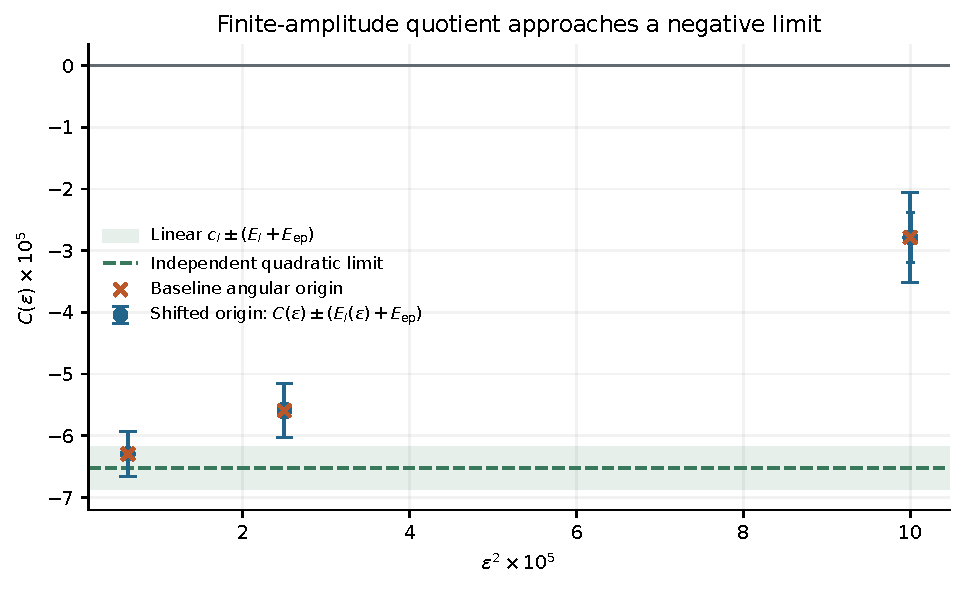
\includegraphics[width=\textwidth]{figures/fig03_nonlinear_quotient.pdf}
\caption{Paired nonlinear quotients approach the quadratic limit. Inner bars give the complete numerical allowance; outer bars add $E_{\mathrm{ep}}$ once, and the horizontal band gives the second linear coefficient and its total allowance. Baseline angular-origin values use the same physical direction and linear baseline.}\label{fig:quotient}
\end{figure}
\begin{figure}[tbp]\centering
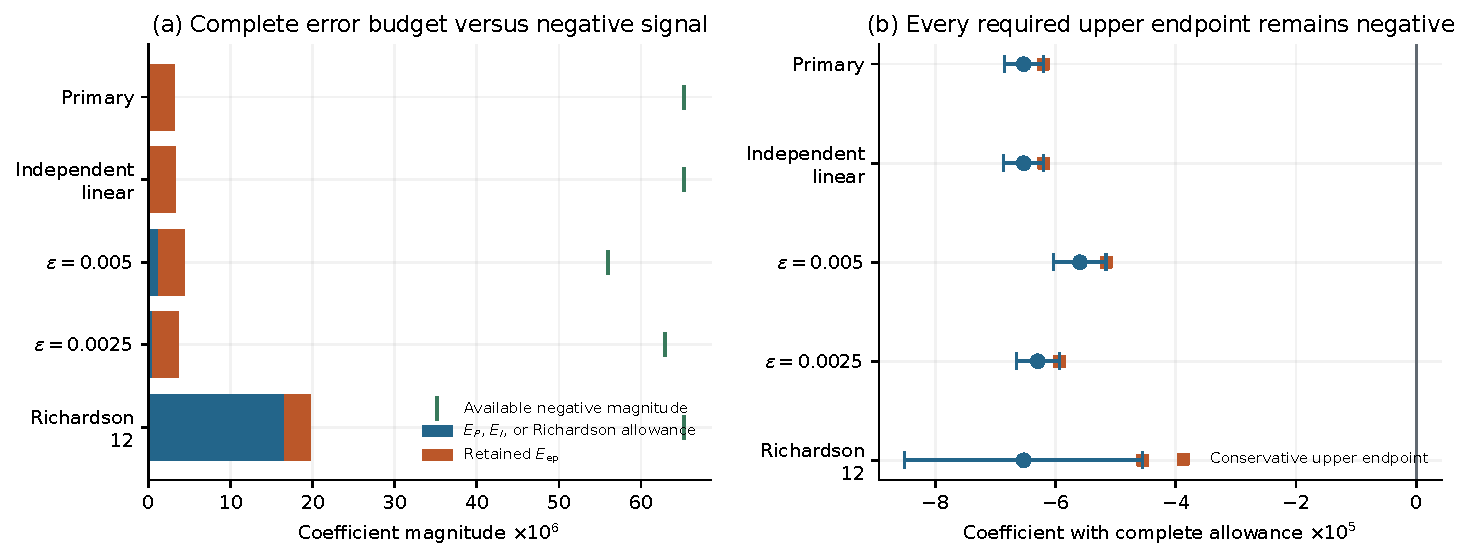
\includegraphics[width=\textwidth]{figures/fig07_error_margin.pdf}
\caption{Negative sign margins after numerical and endpoint allowances. The left panel compares coefficient magnitudes with the two allowances; the right shows centres, complete radii, and empirical upper endpoints. The Richardson value is an extrapolation diagnostic.}\label{fig:margin}
\end{figure}
\FloatBarrier


\section{Methods and numerical uncertainty}\label{sec:methods}
The Gaussian calculation uses the Hermitian amplitude/imaginary-pairing matrix in Eqs.~\eqref{eq:kernelAA}--\eqref{eq:kernelAP}. A second representation linearizes the spatial quasiclassical equations through two Riccati coherence sectors~\cite{Eilenberger1968,Eschrig2000}. Uniform-amplitude, phase Ward, twist--amplitude, current, and zero-field controls establish a common normalization before the spatial comparison.

For the nonlinear response, both causal coherence sectors are expanded in the signed perturbation amplitude, retaining every generated Fourier convolution mode. Spatial averaging takes the zero Fourier coefficient of the retained polynomial; omitted orders and modes remain in the remainder estimates. The normalized anomalous force is integrated along the pairing path and added to the second linear coefficient, avoiding subtraction of large independently accumulated thermodynamic potentials. Sign pairing removes odd orders before absolute errors are formed. Appendix~\ref{app:response} gives the recurrence, both normalization denominators, and the path formula.

The uncertainty construction distinguishes endpoint uncertainty, numerical resolution, and finite-amplitude corrections. The empirical coordinate rectangle is propagated through the background, both coherence sectors, the force, and the temperature prefactor. Low frequencies retain profile-residual and inverse estimates over a connected branch neighbourhood; high frequencies use an analytic complex-amplitude disk and an infinite-frequency tail envelope covering all higher even orders. Neither a finite cutoff nor the retained Fourier polynomial is treated as the full response.

Complete numerical allowances add the linear baseline error, primitive arithmetic estimates, profile and force residuals, path discrepancy, frequency tail, and single- and mixed-refinement contributions. The endpoint allowance is added once. These deterministic additive allowances define the empirical upper endpoints; they are neither statistical confidence intervals nor rigorous interval enclosures. The sign criteria require agreement between representations, negative upper endpoints, and the predefined refinement and source checks. The quadratic total allowances must also be at most one quarter of the coefficient magnitudes.

The angular-origin comparison shares the endpoint, second linear baseline, and continuous-domain estimates. It probes angular discretization sensitivity rather than supplying independent physical observations. Exact refinement levels, source allocations, arithmetic tolerances, and complete acceptance accounting appear in Appendices~\ref{app:response}--\ref{app:repro}.


\section{Interpretation and limitations}
The specified endpoint is stationary within the single-wave ansatz but has a descending direction in the larger spatial pairing space. Its positive uniform amplitude curvature does not prevent a coupled finite-wavevector modulation from lowering the energy. Within this reconstructed mean-field model and its empirical uncertainty framework, self-consistency at the restricted endpoint is therefore insufficient to treat it as an available metastable condensate in a bulk diode calculation.

This is an endpoint-specific result. Earlier Rashba theories establish competition between helical and multiple-wavevector states~\cite{Agterberg2007,Dimitrova2007}; our contribution is the matched quadratic and nonlinear exclusion test at the stated two-dimensional endpoint and fixed asymmetry. Parameters from other dimensionalities or equal-density approximations cannot be transferred without matching conventions. Thermodynamic analyses of perfect equilibrium diodes~\cite{Hosur2026} likewise emphasize the full free-energy landscape, but do not determine the present coefficient's sign.

The numerical conclusion is conditional on the adequacy of the retained binary64 primitive estimates, source-domain controls, and convergence allowances. Analytic subtraction, Fourier identities, and tail estimates do not make their floating-point evaluation a directed-rounding certificate. The endpoint coordinates identify our explicit reconstruction; exact correspondence with the numerical state underlying a published figure or every version of the source model is not established.

The evaluated functional is clean, two dimensional, and intraband, with periodic pairing variations at fixed background twist and field. It excludes impurity scattering, orbital screening, boundaries, and independent electromagnetic degrees of freedom. A different ensemble or finite-size admissibility constraint requires its own test. One descending direction excludes local pairing metastability here, but does not identify the most unstable mode, the global minimum, or the extent of any unstable neighbourhood.

The next physical question is which spatial state replaces the endpoint and whether its stable or metastable current branches retain a large diode response. Answering it requires unrestricted pairing solutions and their continuation under current or twist. Switching dynamics, device geometry, and junction transport are additional problems; the present energy differences do not yield an experimental efficiency or nucleation barrier.

\section{Conclusion}
A fixed finite-wavevector variation coupling amplitude and imaginary pairing components lowers the free energy at the reconstructed nearly maximal Rashba diode endpoint. Two quadratic-response representations and a matched nonlinear calculation retain negative empirical upper endpoints after numerical and endpoint allowances are included. This supplies conditional, model-specific evidence that the stated single-wave endpoint fails a necessary condition for local pairing metastability. The replacement condensate and its transport response remain undetermined.

\section*{Data and reproducibility}
The appendix gives exact inputs, response equations, error accounting, and the complete numerical schedule. Saved measurements, numerical source records, code, and a standalone plotting program accompany the editable manuscript. The figures use those saved measurements; no physical calculation was rerun for this presentation.

\FloatBarrier
\appendix
\section{Exact endpoint and perturbation inputs}\label{app:inputs}
These stored floating-point inputs identify the calculation; their full decimal expansions are not claims of physical precision. The reconstructed endpoint centre is
\begin{equation}\label{eq:coords}
 \begin{aligned}
 T_*&=0.051955058120691594,&\quad\Dstar&=1.6925900731329657,\\
 q_*&=0.9791506418402958,&h_*&=1.3985886221312929.
 \end{aligned}
\end{equation}
The empirical uncertainty rectangle has component half-widths
\begin{equation}\label{eq:rho}
 \bm\rho=(1.225571985\times10^{-8},\ 4.011468456\times10^{-8},
 \ 1.061632250\times10^{-7},\ 1.824801669\times10^{-8}).
\end{equation}

The fixed wavevector and Fourier coefficients are
\begin{align}\label{eq:witness}
 K&=0.909013301211145,\\
 v_A&=-0.13502199918443586,\qquad
 v_P=-0.9908426008888789\,i.
\end{align}
Thus
\begin{equation}\label{eq:profile}
 a(x)=-0.270043998368872\cos Kx,\qquad
 b(x)=1.981685201777758\sin Kx.
\end{equation}

Equivalently, $\eta_+=v_A+iv_P\simeq0.8558206017$ and $\eta_-=v_A^*+iv_P^*\simeq-1.1258646001$, with sidebands at $q_*\pm K$.

\begin{table}[tbp]\centering
\caption{Stored central coefficients and allowances. Numerical radii exclude $E_{\mathrm{ep}}=3.1623619986044952\times10^{-6}$, which is added once to obtain each empirical upper endpoint. Full machine-readable records accompany the article.}\label{tab:rawresults}
\begin{tabular}{lrr}\toprule
Quantity & Central coefficient & Numerical radius\\\midrule
Gaussian & $-6.5287829634528\times10^{-5}$ & $5.8505237960874744\times10^{-8}$\\
Second linear & $-6.528782574296713\times10^{-5}$ & $1.6766293751752474\times10^{-7}$\\
$C(0.01)$ & $-2.7863363462\times10^{-5}$ & $4.0957803644\times10^{-6}$\\
$C(0.005)$ & $-5.5932063990\times10^{-5}$ & $1.1726568826\times10^{-6}$\\
$C(0.0025)$ & $-6.2948907422\times10^{-5}$ & $4.4420405631\times10^{-7}$\\
Final Richardson & $-6.528785523193218\times10^{-5}$ & $1.66327681097\times10^{-5}$\\\bottomrule
\end{tabular}
\end{table}

\begin{flushleft}
The control allowance is $2.0319595130\times10^{-7}$. The two Richardson centres are $-6.528829749948777\times10^{-5}$ and $-6.528785523193218\times10^{-5}$. Origin-shift differences at decreasing amplitudes are $2.7802392560\times10^{-9}$, $6.9433639003\times10^{-10}$, and $1.7353873522\times10^{-10}$; their allowed sums of numerical errors are $9.5198562301\times10^{-6}$, $2.6777244933\times10^{-6}$, and $9.7165279423\times10^{-7}$.
\end{flushleft}

\section{Functional consistency and endpoint derivatives}\label{app:functional}
\subsection{Amplitude and twist differentiation}
Equation~\eqref{eq:uniformF} gives $\partial_D\Omega=D/\Omega$ and therefore
\begin{equation}
 \partial_Df=2D\ln T+2\pi TD\sum_{n\ge0}
 \left[\frac{2}{\omega_n}-\sum_\lambda W_\lambda
 \operatorname{Re}\av{\Omega^{-1}}\right].
\end{equation}
At $h=q=0$, $\sum_\lambda W_\lambda=2$ and $\Omega=\sqrt{\omega_n^2+D^2}$. Dividing by $2D$ yields
\begin{equation}
 \ln T+2\pi T\sum_{n\ge0}
 \left(\frac{1}{\omega_n}-\frac{1}{\sqrt{\omega_n^2+D^2}}\right)=0,
\end{equation}
the standard transition-temperature-subtracted uniform gap equation in these units. A spurious extra factor of $T$ multiplying the logarithm would fail this check. Source plotting conventions also require care: where the source uses $\xi=v_F/|\Delta_q|$ and scales field by $|\Delta_q|$, its plotted momentum and field correspond to $q/D$ and $h/D$, rather than the $\Tc$-scaled $q,h$ used in this manuscript. The reconstructed coordinates must not be directly identified with those source-figure abscissae. The derivation also distinguishes $N_0$ from the total density of states.

For the twist, $\partial_qz=(i/2)\cos\theta$ and $\partial_q\Omega=(z/\Omega)\partial_qz$. Since $\operatorname{Re}(iX)=-\operatorname{Im}X$ and $\operatorname{Re}\partial_qz=0$, differentiating the negative determinant contribution gives Eq.~\eqref{eq:current}. This fixes the current/free-energy normalization without fitting a response prefactor to the final negative mode.

\subsection{Total versus partial endpoint derivatives}
Set $s=D'(q)=-f_{Dq}/f_{DD}$. Along the gap branch,
\begin{equation}
 g'=f_q,\qquad
 g''=f_{qq}-\frac{f_{qD}^2}{f_{DD}},\qquad
 g'''=f_{qqq}+3f_{qqD}s+3f_{qDD}s^2+f_{DDD}s^3.
\end{equation}
These are total derivatives after amplitude relaxation. Replacing them by fixed-$D$ derivatives would locate a different object. The endpoint calculation uses a four-variable root and gives an infinity-norm condition estimate of about $124.636$. Its coordinate uncertainty includes numerical refinements and solver effects rather than being identified with the central residual alone.

The central dimensionless free energy is $f_*=-0.63217093656$. The saved uniform amplitude derivative and twist derivative are near zero, but $f_{qq}\simeq0.08498845757$ is positive: it is the relaxed combination $g''$, not $f_{qq}$ by itself, that vanishes. This illustrates the importance of distinguishing a restricted variable change from the relaxed branch condition. The spatial perturbation is a further, different enlargement of the variation space.

\section{Detailed response construction}\label{app:response}
\subsection{Two representations of the local pairing response}
The primary response is the second variation of the source-compatible mean-field functional. In the background-helix gauge, write $p=\bm K\cdot\widehat{\bm k}$ and $L=4\Omega^2+p^2$, using dimensionless $v_F=1$. In the Cartesian amplitude/imaginary-pairing basis the Hermitian $2\times2$ matrix is
\begin{align}\label{eq:kernelAA}
 M_{AA}(\bm K)&=2\ln T+2\pi T\sum_{n\ge0}\left[\frac{2}{\omega_n}
 -\sum_\lambda W_\lambda\operatorname{Re}\av{\frac{4z^2}{\Omega L}}\right],\\
 M_{PP}(\bm K)&=2\ln T+2\pi T\sum_{n\ge0}\left[\frac{2}{\omega_n}
 -\sum_\lambda W_\lambda\operatorname{Re}\av{\frac{4\Omega}{L}}\right],\label{eq:kernelPP}\\
 M_{AP}(\bm K)&=-4\pi iT\sum_{n\ge0,\lambda}W_\lambda
 \av{p\operatorname{Im}\left(\frac{z}{\Omega L}\right)},
 \qquad M_{PA}=M_{AP}^*.\label{eq:kernelAP}
\end{align}
These are derived source-compatible response equations, not quotations from the source paper. The band, angular, and ultraviolet conventions are those in Section~\ref{sec:model}. The response coefficient is $\bm v^\dagger M\bm v$ for the physical harmonics in Eqs.~\eqref{eq:ab}--\eqref{eq:witness}.

The radial reduction in the underlying two-propagator calculation uses
\begin{equation}\label{eq:radial}
 \int_{-\infty}^{\infty}\frac{\dd\xi}{A_+A_-}
 =\frac{2\pi}{\Omega(4\Omega^2+p^2)},\qquad
 \int_{-\infty}^{\infty}\frac{\xi^2\dd\xi}{A_+A_-}
 =\frac{\pi}{2\Omega},\qquad
 A_\pm=(\xi\pm p/2)^2+\Omega^2.
\end{equation}
The analytic branch prescription accompanies these identities. The matrix has amplitude and imaginary-pairing vertices corresponding to $\tau_x$ and $-\tau_y$ in the Nambu convention of the constructed functional. An arbitrary positive prefactor would leave the sign unchanged, but would fail the required quantitative comparison with nonlinear free-energy differences.

The second response representation uses the spatial quasiclassical equations, expressed through two Riccati coherence sectors. Quasiclassical transport and coherence parametrizations are established tools~\cite{Eilenberger1968,Eschrig2000}; the two-sector expansion, source-domain controls, and normalized-force implementation described below specify the representation used in this calculation. Both representations share the physical model and endpoint inputs.

\subsection{Normalization and source controls before the spatial test}
At $K=0$, the matrix must reproduce the uniform Cartesian second variations,
\begin{equation}\label{eq:ward}
 M_{AA}(0)=f_{DD},\qquad M_{PP}(0)=\frac{f_D}{D}.
\end{equation}
The second identity is the phase Ward control. The measured residual is retained rather than replacing the right-hand side by zero by hand. The mixed response at small $K$ is checked against the twist--amplitude derivative in the same normalization. Additional retained controls compare the raw source response, the signed force, current and free-energy derivatives, zero-field limits, and Hermiticity.

\subsection{Periodic Riccati expansion with complete Fourier support}
For one helicity, trajectory, and positive Matsubara frequency, the uniform coherence amplitude is
\begin{equation}
 a_0=\frac{D}{z+\Omega}.
\end{equation}
At signed physical perturbation amplitude $\beta$, write the two coherence sectors as
\begin{equation}\label{eq:riccati}
 A_\beta=a_0+\beta U_\beta,\qquad
 B_\beta=a_0+\beta V_\beta.
\end{equation}
Both sectors use the same causal $z$. The second sector reverses transport and conjugates the prescribed pairing profile; it does not replace $z$ by $z^*$. This distinction is necessary when the field and phase twist produce a complex Matsubara shift.

Expanding $U_\beta=\sum_{k\ge0}\beta^k U_k$, the Fourier inverse has denominator $2\Omega+imp$. With $\mathcal L_m=2\Omega+imp$, the recurrence can be written
\begin{align}\label{eq:recurrence}
 \mathcal L U_0&=\eta-a_0^2\eta^*,\\
 \mathcal L U_k&=-2a_0\eta^*U_{k-1}
 -D\!\sum_{i+j=k-1}U_iU_j
 -\eta^*\!\sum_{i+j=k-2}U_iU_j\quad(k\ge1).
\end{align}
The $V$ sector uses the conjugate profile and the opposite transport denominator. Empty sums vanish. At each order, every convolution mode generated by the recurrence is retained; for a first-harmonic forcing the support grows to $|m|\le k+1$. Products are evaluated by full finite Fourier convolution rather than by a spatial collocation grid that could fold modes back into the retained range.

The spatial mean of the retained polynomial is exactly its zero Fourier coefficient. ``Exact'' here describes the finite Fourier averaging identity, not an exact arithmetic evaluation or a claim that the infinite response is a finite polynomial. Omitted perturbative orders and their Fourier content remain in the residual and analytic remainder estimates.

\subsection{Normalized anomalous force and energy-path integration}
The normalized force has two denominator factors. Defining
\begin{equation}
 Q=1+a_0^2,\qquad h_\beta=\beta a_0(U_\beta+V_\beta)+\beta^2U_\beta V_\beta,
\end{equation}
the divided anomalous response is
\begin{equation}\label{eq:dividedforce}
 \mathcal A_\beta=
 \frac{2\left(U_\beta-a_0^2V_\beta-\beta a_0U_\beta V_\beta\right)}
 {Q\left(Q+h_\beta\right)}.
\end{equation}
The finite denominator $Q+h_\beta$ and the background factor $Q$ both enter the force estimates. Bounding only one would not control the normalized physical response. The scalar force contribution is the real spatial zero mode of $\eta^*\mathcal A_\beta$, denoted $\mathcal G_\beta$.

Instead of subtracting two independently accumulated large thermodynamic potentials, the nonlinear coefficient is assembled as a correction to the matched linear coefficient:
\begin{equation}\label{eq:path}
 C(\epsilon)=c_0-\pi T\sum_{n\ge0,\lambda}W_\lambda
 \av{\sum_{\sigma=\pm1}\int_0^1
 t\left[\mathcal G_{\sigma t\epsilon}-\mathcal G_0\right]\dd t}.
\end{equation}
The log and $1/\omega_n$ counterterms cancel in this correction; they are already present in the second linear baseline. The source-dependent $\pi T$ prefactor remains explicit. The anchor's numerical allowance is included once in the complete quotient error.

Path integration is checked against closed polynomial moments. A term proportional to $\beta^k$ contributes the moment $\int_0^1 t^{k+1}\dd t=1/(k+2)$. The paired signs remove odd orders before error magnitudes are formed. Gaussian path-node refinement is retained as a numerical control, and the path-polynomial discrepancy is propagated rather than assumed to vanish.

The norm used in analytic majorants is the Fourier $\ell^1$ norm of the forcing profile. It bounds convolution and remainder growth; it is not an additional denominator in Eq.~\eqref{eq:paired}. For the normalized two-component witness, the spatial mean of $|\eta|^2$ is two. Dividing the final energy quotient by that norm would change the normalization and destroy the match to $\bm v^\dagger M\bm v$.

\subsection{Low-frequency coverage, source uncertainty, and connected branches}
Low positive Matsubara frequencies are the numerically delicate part of the calculation. Frequencies $n<32$ use explicit source-coefficient radii, complete omitted-profile residuals, the full normalization identity, and inverse estimates that cover both the retained finite-mode block and the infinite high-mode remainder. Sixteen signed-$\beta$ cells cover $[-0.01,0.01]$; the calculated common profile remainder cap is $0.001$, with a high-mode split index of 12.

The bounds preserve a common connected uniqueness neighbourhood for the two coherence sectors and the signed amplitudes. This guards against accepting a different algebraic branch at one amplitude. Continuous angular-domain estimates cover the stated endpoint rectangle and signed-$\beta$ interval. The two angular-origin calculations share these domain estimates and the same linear baseline; this dependence is included when interpreting their comparison.

The source uncertainty is a rectangle in all four coordinates in Eq.~\eqref{eq:coords}. Its effects are propagated through the uniform background, both Riccati sectors, the normalized force, and the temperature prefactor. Evaluating only the centre, or only a few corners, would not establish the documented domain coverage. A coordinate stored exactly as a binary64 number is still the centre of a physically uncertain reconstructed state.

The endpoint-error allocation uses $\Eep$ once. The linear endpoint-variation estimate occupies $9.9246651098\times10^{-7}$; the remaining nonlinear source-correction allowance is $2.1698954876\times10^{-6}$. These add to $\Eep$. The measured nonlinear source radii are smaller than the available nonlinear allowance. They are not treated as independent random variables to be combined in quadrature with the endpoint allowance.

\subsection{High frequencies and the complete omitted Matsubara tail}
For $n\ge32$, a source-uniform complex-$\beta$ disk of radius $r=0.1$ supports analytic remainder estimates in addition to the explicitly computed finite-amplitude correction. The omitted-frequency estimate includes every higher even perturbative order after sign pairing. The tail is not set to zero at the largest computed frequency.

For a source-uniform force majorant of the form $|\mathcal G_\beta-\mathcal G_0|\le C_f/\omega^3$ on the disk, the retained paired envelope has the form
\begin{equation}\label{eq:tail}
 B_{\mathrm{tail}}\le 2\pi T_{\max} C_f
 \frac{(\epsilon/r)^2}{1-(\epsilon/r)^2}
 \left[\frac{1}{w^3}+\frac{1}{4\pi T_{\min}w^2}\right],
 \qquad w=(2N_\omega+1)\pi T_{\min},
\end{equation}
with the calculated arithmetic allowance added. The geometric factor retains all omitted even orders. $C_f$ is obtained from the source-uniform two-sector, two-pole contraction estimates, rather than fitted to a decreasing sequence of observed tail values.

At $N_\omega=512$, the saved infinite-frequency quotient-tail envelopes are approximately $1.5156907408\times10^{-6}$, $3.7607439433\times10^{-7}$, and $9.3842953931\times10^{-8}$ at $\epsilon=0.01,0.005,0.0025$. Their amplitude dependence is consistent with the correction's leading even order. They are components of the complete error budget, not the complete uncertainty by themselves.

\subsection{Five refinement axes and all mixed pairs}
A configuration is calculated as
\begin{equation}\label{eq:config}
 (J,N_\omega,N_\theta,P,N_t).
\end{equation}
The axes and their three levels are listed in Table~\ref{tab:levels}. $J$ is the retained profile expansion degree; $2P$ is the retained force expansion degree; $N_t$ controls the path rule. The angular rules use one common origin to preserve their nested hierarchy. They do not rotate the physical $q$, $\bm h$, or $\bm K$.

\begin{table}[tbp]\centering
\caption{\textbf{Numerical refinement levels.} The finest configuration is $(16,512,64,8,8)$. The schedule contains the fine centre, two lower levels along each axis, and two levels for each of ten mixed pairs, giving $1+10+20=31$ configurations. Three perturbation amplitudes give 93 rows.}\label{tab:levels}
\begin{tabular}{llrrr}\toprule
Axis & Meaning & Coarse & Medium & Fine\\\midrule
$J$ & Profile perturbation degree &8&12&16\\
$N_\omega$ & Explicit positive Matsubara frequencies &128&256&512\\
$N_\theta$ & Angular nodes &16&32&64\\
$P$ & Half the force perturbation degree &4&6&8\\
$N_t$ & Path quadrature nodes &2&4&8\\\bottomrule
\end{tabular}
\end{table}

For an axis, let $d_1$ be the medium-minus-coarse change and $d_2$ the fine-minus-medium change. The predefined rule requires $|d_2|\le0.75|d_1|+b_{\mathrm{noise}}$, with a same-sign condition unless the change is noise sized. The calculated axis allowance is constructed from the final change and the row error radii, including the form $4(|d_2|+b_1+b_2)+b_2$. Convergence ratios alone are insufficient when cancellation drives a difference close to the primitive noise floor.

Mixed contrasts detect interactions between refinements. They compare jointly changed settings with their individually changed counterparts at two levels for each axis pair. All ten pairs are tested and their allowances included. This avoids assigning the entire error to separate one-dimensional differences when, for example, profile and angular refinements interact.

The complete quotient allowance includes the second linear anchor, spatial/profile remainder, primitive arithmetic and normalized-force defects, path integration, the infinite-frequency tail, the five axis allowances, and the ten mixed allowances. It is added as an absolute radius, not interpreted as a statistical variance. The amplitude hierarchy is separately checked with its predefined contraction factor of $0.5$ plus propagated noise. The Richardson check has its own complete allowance.

\subsection{Numerical criteria and angular-origin comparison}
The local quadratic test requires both source-inclusive upper bounds to be negative, the primary and independent total radii to be at most one quarter of the respective coefficient magnitudes, and representation agreement within $E_{\mathrm P}+\EI$. The source controls must fit inside the endpoint-error allocation. The nonlinear sign test additionally requires $C_1$ and $C_2$ to remain negative beyond their complete numerical and endpoint allowances. Source and branch controls, the complete schedule, refinement and amplitude rules, tail coverage, and origin agreement are required as applicable. Unresolved numerical checks are inconclusive; they are not physical evidence for either sign.

The fresh confirmation uses
\begin{equation}\label{eq:origin}
 \theta_j=\frac{2\pi j}{N_\theta}+\phi_0,\qquad
 \phi_0=\frac{\pi\sqrt5}{256}.
\end{equation}
Every angle-dependent nonlinear response in the 93-row schedule was recomputed on this origin. Its comparison with the baseline-origin calculation shares the same physical state, linear coefficient, and continuous-domain estimates. The comparison therefore probes discretization sensitivity of the fixed direction; it is not statistical replication.

\subsection{Arithmetic and computational cost}
The calculations use binary64 real and complex128 arithmetic. Primitive error estimates include an empirical floor of $10^{-12}$; recurrence and normalization residuals are required to be at most $10^{-10}$. These tolerances enter the error estimates and are not a replacement for controlling frequency tails or endpoint-coordinate uncertainty. Vectorized coefficient contractions accelerate the recurrence and majorant calculations without changing the model or the retained Fourier support.

The complete shifted-origin calculation requires $12751.5790$ seconds of calculation CPU time and $14348.2845$ seconds elapsed, approximately 3.54 CPU hours and 3.99 elapsed hours. These costs refer to the 606208 two-sector expansions and associated numerical processing. The schedule comprises 606208 two-sector expansion nodes: 1184 at each of 512 explicit positive Matsubara frequencies. The stored angular origin is $0.02744068254312784$ radians.


\section{Detailed error accounting and acceptance arithmetic}\label{app:errors}
\subsection{Additive error decomposition}
For each amplitude, let $E_{\mathrm{fine}}$ denote the finest row's complete coefficient radius, including the second linear baseline uncertainty and explicit nonlinear components. The final complete allowance is
\begin{equation}\label{eq:EIassembled}
 E_C=E_{\mathrm{fine}}+\sum_{a=1}^5E_a
 +\sum_{1\le a<b\le5}E_{ab}.
\end{equation}
The original endpoint/source allowance $\Eep$ is then added once for the sign test. The row-specific nonlinear source radius is checked against its allocated source budget. Adding it again on top of the full $\Eep$ would double count that coverage.

At the finest row, the explicit numerical correction radius is the sum of tail, primitive, normalized-force residual, path-polynomial, and spatial terms. The aggregate quotient radius must also account for the second linear baseline and the observed refinement hierarchy. Table~\ref{tab:errorbreakdown} shows the resulting decomposition. A zero calculated spatial term applies to the retained finite-polynomial accounting; omitted modes/orders are covered by the residual and analytic estimates, not asserted absent from the physical response.

\begin{table}[tbp]\centering
\caption{Nonlinear numerical allowance decomposition. Endpoint allowance $E_{\mathrm{ep}}=3.1623619986\times10^{-6}$ is added separately and once for the sign test. Values use the normalized quotient units.}\label{tab:errorbreakdown}
\begin{tabular}{rrrrrr}\toprule
$\epsilon$ & Fine row & Five axes & Ten mixed & Total $E_C$ \\\midrule
0.0100 & $1.683720\times10^{-6}$ & $2.386198\times10^{-6}$ & $2.586194\times10^{-8}$ & $4.095780\times10^{-6}$ \\
0.0050 & $5.441040\times10^{-7}$ & $6.026909\times10^{-7}$ & $2.586194\times10^{-8}$ & $1.172657\times10^{-6}$ \\
0.0025 & $2.618726\times10^{-7}$ & $1.564696\times10^{-7}$ & $2.586194\times10^{-8}$ & $4.442041\times10^{-7}$ \\
\bottomrule\end{tabular}\end{table}


The mixed checks use saved contrasts $m_1,m_2$ and corresponding row-noise allowances $b_1,b_2$. The convergence heatmap shows the maximum of
\begin{equation}
 \frac{|m_2|}{0.75|m_1|+b_1+b_2},\qquad
 \frac{|m_2|}{0.25\sum_{\ell=1}^5E_\ell+b_2}.
\end{equation}
A value below one satisfies both magnitude conditions represented in the panel. The axis and amplitude hierarchies also retain their respective sign/noise rules; colour alone is not a substitute for the complete numerical checks.

\subsection{Source and amplitude uncertainty are distinct}
The endpoint coordinate uncertainty affects both the background linear coefficient and the nonlinear correction. Their documented source budgets are assigned so that the total stays within the original $\Eep$. Refinement errors instead measure resolution sensitivity under the fixed source domain. The two should not be combined as uncorrelated Gaussian variables.

Similarly, the difference between $C(0.005)$ and $C(0.0025)$ is primarily a finite-amplitude correction, not a sampling uncertainty. The extrapolation removes its leading even order under an analytic expansion. The complete Richardson allowance remains large enough that the sign conclusion does not depend on claiming its central-value precision as certified precision.

\subsection{Numerical consistency criteria}
The retained numerical consistency criteria are: source controls; complete axis and mixed hierarchy; complete nonlinear $C_1$ negativity; complete nonlinear $C_2$ negativity; complete Richardson negativity; complete schedule; amplitude hierarchy; normalization-control adequacy; linear-response negativity; cross-representation agreement; quarter-error rule; shifted-origin agreement; and source-budget adequacy. All of these criteria are required together for the stated conclusion. 

The formal stability implication and its numerical premise should remain separate. Conditional on an actual $c<0$ and the usual differentiability of the functional, Eq.~\eqref{eq:descent} excludes a local minimum. The present calculation supplies empirical numerical evidence for that premise in the stated model; it does not prove that all primitive errors have been enclosed for every real input by directed rounding.

\section{Reproduction recipe and complete configuration table}\label{app:repro}
The numerical calculation can be reconstructed from the physical and numerical definitions in this article. A reproduction must use the same normalization throughout; resolving a negative sign with a mismatched overall factor would not reproduce the stated coefficients.

\begin{enumerate}
\item Fix $\widetilde\alpha=1/4$, the causal positive-frequency branch, and the dimensionless units in Eq.~\eqref{eq:units}. Evaluate the uniform functional with its transition-temperature subtraction and the infinite-frequency remainder.
\item Solve the four endpoint equations in Eq.~\eqref{eq:endpoint}, using total derivatives along the amplitude-relaxed branch. Check the two coexistence minima and intermediate stationary point, positive amplitude curvature, and positive relaxed quartic. Propagate the coordinate rectangle in Eq.~\eqref{eq:rho}.
\item Fix $K,v_A,v_P$ in Eq.~\eqref{eq:witness}. Evaluate Eqs.~\eqref{eq:kernelAA}--\eqref{eq:kernelAP} and the zero-wavevector/current normalization checks. Independently evaluate the linearized Riccati response, including its full numerical error estimate.
\item For each angular rule and positive Matsubara frequency, expand both causal Riccati sectors using Eq.~\eqref{eq:recurrence}. Keep every generated Fourier convolution mode. Evaluate the normalized force in Eq.~\eqref{eq:dividedforce}, controlling both denominator factors and the omitted profile remainder.
\item Integrate the paired nonlinear correction in Eq.~\eqref{eq:path}, with the two signs and the three amplitudes. Check polynomial path moments, the source rectangle, signed-amplitude branch continuity, low-frequency residual estimates, and the complex-amplitude disk. Include the complete omitted-frequency envelope in Eq.~\eqref{eq:tail}.
\item Evaluate the 31 configurations in Table~\ref{tab:configurations}; construct single-axis changes, all ten mixed contrasts, amplitude contraction and Richardson values. Add the numerical allowances as in Eq.~\eqref{eq:EIassembled}, and add the endpoint allowance once. Compare the primary and second linear coefficients and test the strict negative upper endpoints.
\item Repeat the nonlinear angular calculation with the common shifted origin in Eq.~\eqref{eq:origin}. Compare the resulting coefficients against the sum of complete numerical allowances. This final step tests angular sensitivity while sharing the fixed state and linear baseline.
\end{enumerate}

The equations specify the functional, perturbation, expansion, force, integration path, numerical hierarchy, error composition and sign criterion. They do not convert the empirical primitive estimates into validated interval arithmetic: that limitation remains part of the reproducible result. A rigorously certified reproduction would additionally require outward-rounded primitive and accumulation bounds over the entire parameter domain.



Table~\ref{tab:configurations} reports every configuration and the three corresponding central quotients. All physical inputs are given in Eqs.~\eqref{eq:coords}, \eqref{eq:rho}, and \eqref{eq:witness}; the numerical levels are in Table~\ref{tab:levels}. Central-value digits allow numerical comparison; the appropriate uncertainty remains the complete numerical allowance plus endpoint allowance in Table~\ref{tab:nonlinear}.
\small
\begin{longtable}{rrrrrrrr}
\caption{Shifted-origin configurations and central quotients in units of $10^{-5}$. Settings follow Eq.~\eqref{eq:config}; the finest configuration is $(16,512,64,8,8)$.}\label{tab:configurations}\\
\toprule $J$ & $N_\omega$ & $N_\theta$ & $P$ & $N_t$ & $C(.01)$ & $C(.005)$ & $C(.0025)$\\\midrule\endfirsthead
\toprule $J$ & $N_\omega$ & $N_\theta$ & $P$ & $N_t$ & $C(.01)$ & $C(.005)$ & $C(.0025)$\\\midrule\endhead
\bottomrule\endfoot
8 & 128 & 64 & 8 & 8 & -2.79025510 & -5.59418609 & -6.29513566\\
8 & 512 & 16 & 8 & 8 & -2.16735454 & -5.43841537 & -6.25619014\\
8 & 512 & 64 & 4 & 8 & -2.78633635 & -5.59320640 & -6.29489074\\
8 & 512 & 64 & 8 & 2 & -2.78635207 & -5.59320738 & -6.29489080\\
8 & 512 & 64 & 8 & 8 & -2.78633635 & -5.59320640 & -6.29489074\\
12 & 256 & 64 & 8 & 8 & -2.78712183 & -5.59340277 & -6.29493983\\
12 & 512 & 32 & 8 & 8 & -2.72765934 & -5.57852796 & -6.29122056\\
12 & 512 & 64 & 6 & 8 & -2.78633635 & -5.59320640 & -6.29489074\\
12 & 512 & 64 & 8 & 4 & -2.78633635 & -5.59320640 & -6.29489074\\
12 & 512 & 64 & 8 & 8 & -2.78633635 & -5.59320640 & -6.29489074\\
16 & 128 & 16 & 8 & 8 & -2.17127330 & -5.43939506 & -6.25643506\\
16 & 128 & 64 & 4 & 8 & -2.79025510 & -5.59418609 & -6.29513566\\
16 & 128 & 64 & 8 & 2 & -2.79027083 & -5.59418707 & -6.29513573\\
16 & 128 & 64 & 8 & 8 & -2.79025510 & -5.59418609 & -6.29513566\\
16 & 256 & 32 & 8 & 8 & -2.72844482 & -5.57872433 & -6.29126965\\
16 & 256 & 64 & 6 & 8 & -2.78712183 & -5.59340277 & -6.29493983\\
16 & 256 & 64 & 8 & 4 & -2.78712183 & -5.59340277 & -6.29493983\\
16 & 256 & 64 & 8 & 8 & -2.78712183 & -5.59340277 & -6.29493983\\
16 & 512 & 16 & 4 & 8 & -2.16735454 & -5.43841537 & -6.25619014\\
16 & 512 & 16 & 8 & 2 & -2.16735001 & -5.43841509 & -6.25619012\\
16 & 512 & 16 & 8 & 8 & -2.16735454 & -5.43841537 & -6.25619014\\
16 & 512 & 32 & 6 & 8 & -2.72765934 & -5.57852796 & -6.29122056\\
16 & 512 & 32 & 8 & 4 & -2.72765934 & -5.57852796 & -6.29122056\\
16 & 512 & 32 & 8 & 8 & -2.72765934 & -5.57852796 & -6.29122056\\
16 & 512 & 64 & 4 & 2 & -2.78635207 & -5.59320738 & -6.29489080\\
16 & 512 & 64 & 4 & 8 & -2.78633635 & -5.59320640 & -6.29489074\\
16 & 512 & 64 & 6 & 4 & -2.78633635 & -5.59320640 & -6.29489074\\
16 & 512 & 64 & 6 & 8 & -2.78633635 & -5.59320640 & -6.29489074\\
16 & 512 & 64 & 8 & 2 & -2.78635207 & -5.59320738 & -6.29489080\\
16 & 512 & 64 & 8 & 4 & -2.78633635 & -5.59320640 & -6.29489074\\
16 & 512 & 64 & 8 & 8 & -2.78633635 & -5.59320640 & -6.29489074\\
\end{longtable}
\normalsize


\FloatBarrier
\section{Diagnostic figures}
\begin{figure}[tbp]\centering
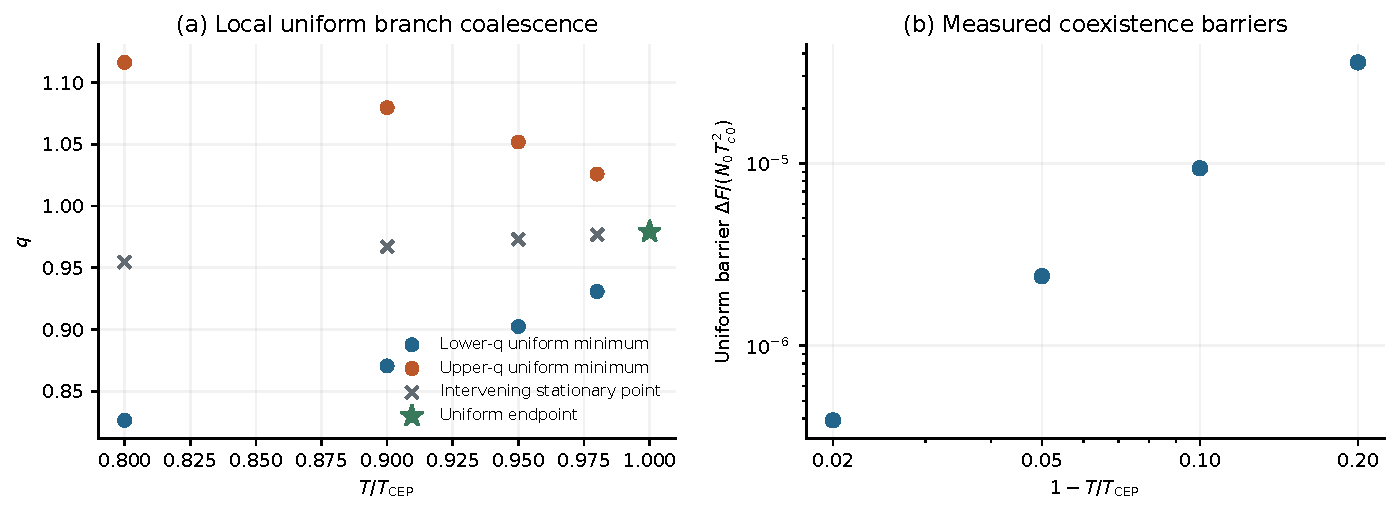
\includegraphics[width=\textwidth]{figures/fig01_endpoint_topology.pdf}
\caption{Restricted uniform endpoint topology. Samples at four temperatures between $0.80T_*$ and $0.98T_*$ show the two coexistence minima and intervening stationary point; the right panel gives uniform barriers. The field varies along coexistence, and connecting samples does not establish a fixed-field scan or fitted critical law.}\label{fig:endpoint}
\end{figure}
\begin{figure}[tbp]\centering
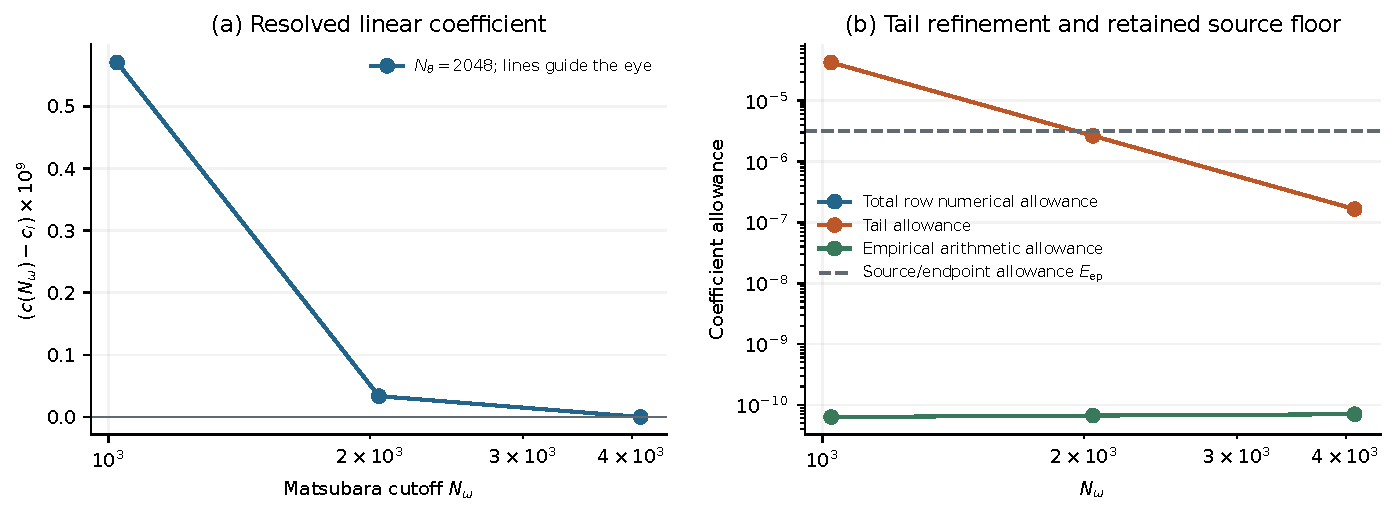
\includegraphics[width=\textwidth]{figures/fig02_linear_qualification.pdf}
\caption{Second quadratic-response representation under frequency refinement at $N_\theta=2048$. Coefficients are measured relative to the finest row; the right panel separates row numerical, tail, and primitive-arithmetic radii from the endpoint allowance. The final allowance also includes single- and mixed-refinement contributions.}\label{fig:linear}
\end{figure}
\begin{figure}[tbp]\centering
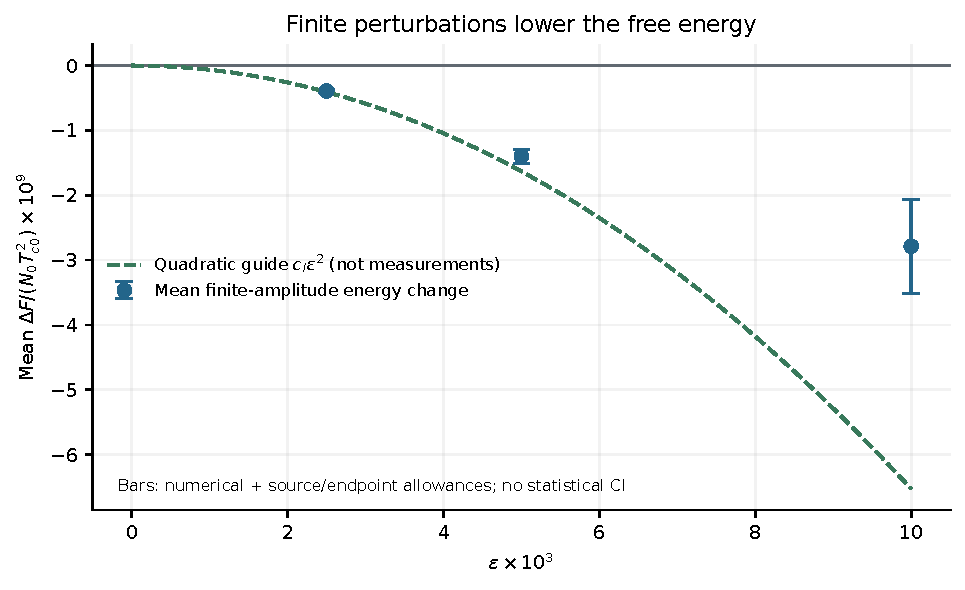
\includegraphics[width=\textwidth]{figures/fig04_energy_descent.pdf}
\caption{Paired mean energy change $\overline{\delta f}=\epsilon^2C$ in units of $N_0\Tc^2$, reconstructed from the computed quotients with radius $\epsilon^2(E_C+E_{\mathrm{ep}})$. The dashed $\cI\epsilon^2$ curve is a quadratic guide. A negative paired mean ensures a descending signed member without assigning equal lowering to both signs.}\label{fig:energy}
\end{figure}
\begin{figure}[tbp]\centering
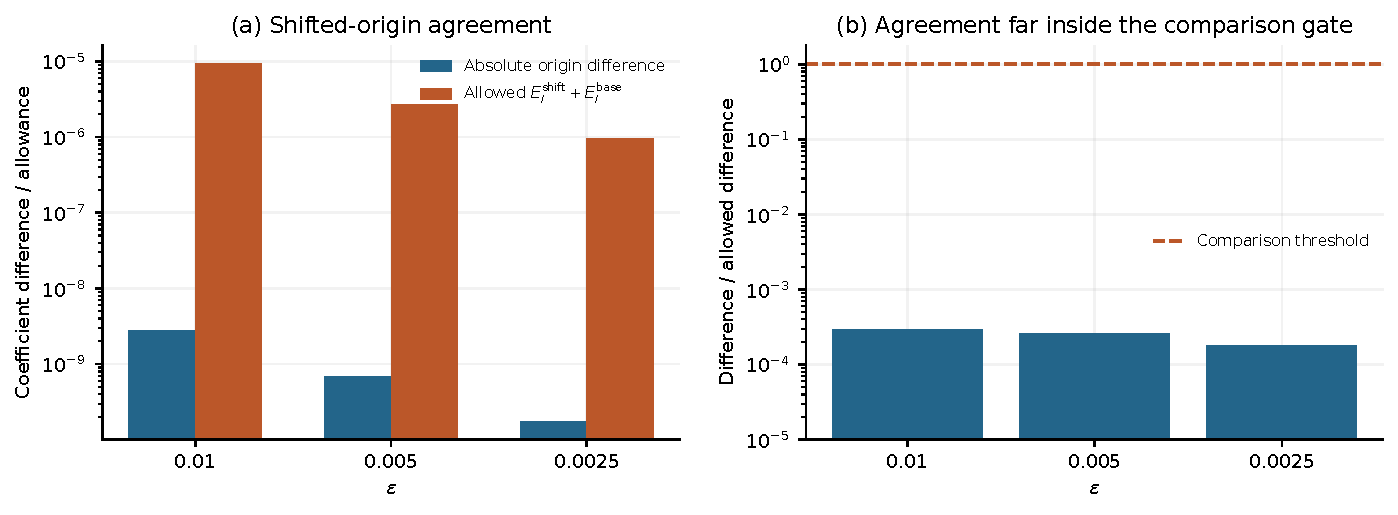
\includegraphics[width=\textwidth]{figures/fig05_origin_agreement.pdf}
\caption{Angular-origin sensitivity. Absolute quotient differences after shifting the origin by $\pi\sqrt5/256$ are smaller than the sum of complete numerical allowances. The comparison shares the physical direction, linear baseline, and domain estimates; common endpoint uncertainty is excluded from the difference allowance.}\label{fig:origin}
\end{figure}
\begin{figure}[tbp]\centering
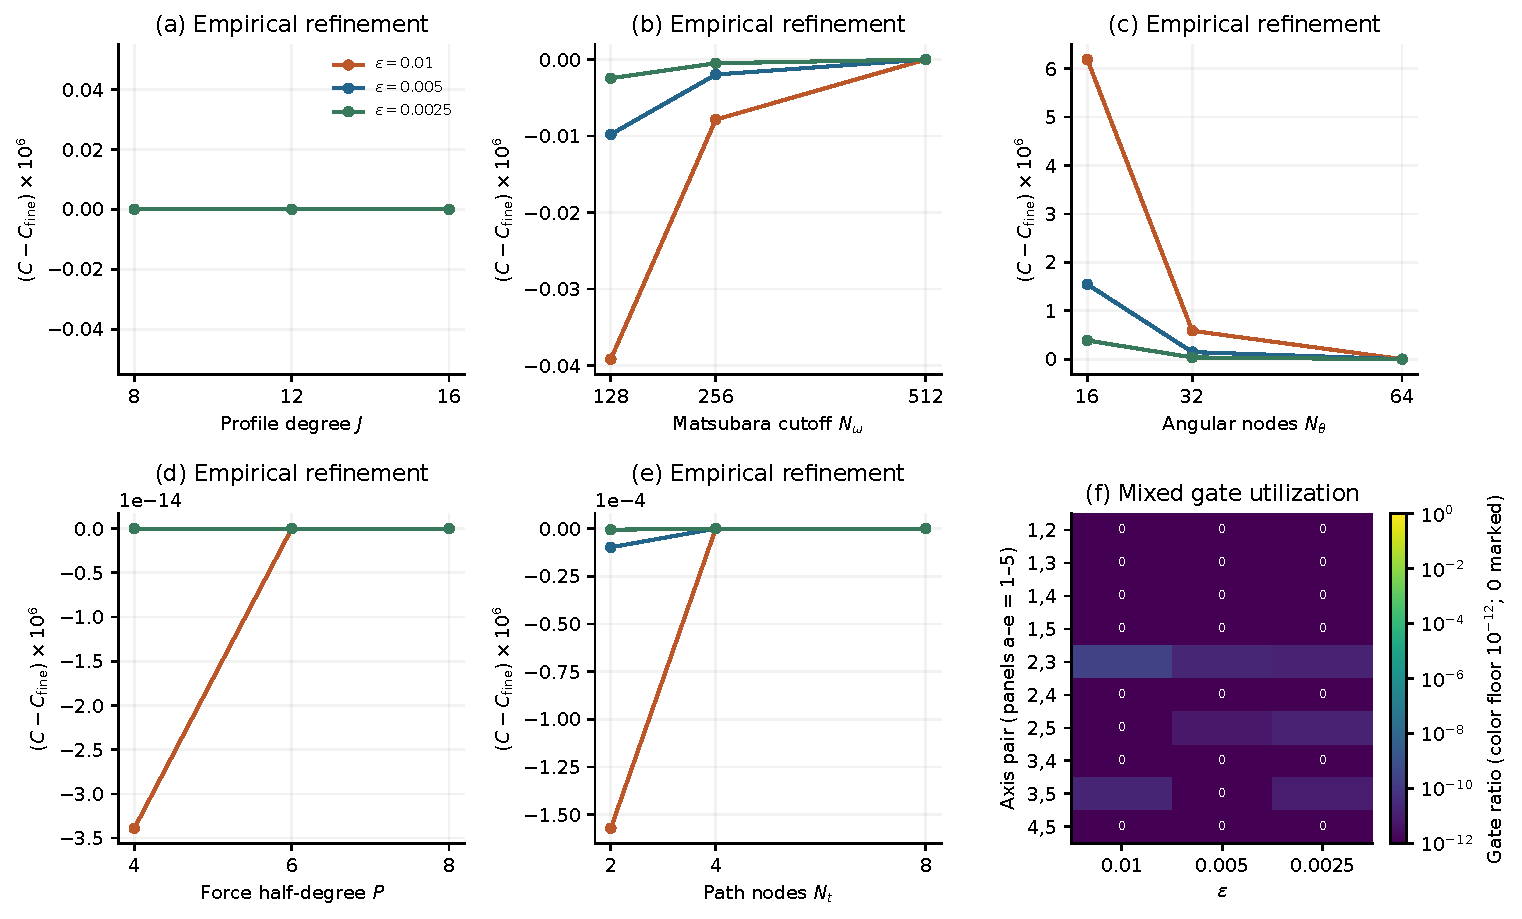
\includegraphics[width=\textwidth]{figures/fig06_axis_mixed_convergence.pdf}
\caption{Single- and mixed-refinement diagnostics. Single-axis changes relative to the finest row are shown in units of $10^{-6}$, with axis definitions in Table~\ref{tab:levels}. The final panel gives the larger utilization of the two inequalities in Appendix~\ref{app:errors}; values below $10^{-12}$ share the lowest colour, and computed exact zeros are marked.}\label{fig:axes}
\end{figure}
\FloatBarrier


\begingroup\raggedright
\bibliographystyle{unsrtnat}
\bibliography{references}
\endgroup
\end{document}
